\bodychapter{Pairings}
\label{chp:pair}

One area of cryptography that we have yet to touch on is \textit{pairing based
    cryptography}.
Pairings are bilinear forms over specific points on an elliptic curve (more on
    that in a moment), and were actually first used in cryptography to attack
    cryptosystems rather than implement them---see Chapter \ref{chp:app} for
    more details.
In this chapter we'll discuss the mathematics of pairings, beginning with the
    necessary background information.
From there, we'll discuss one way to compute an important function, dubbed a
    \textit{Miller function}, over a binary Edwards curve.
Finally, we'll discuss some interesting directions for future work, including a
    preliminary result that may help pave the way.

\bodysection{Background}

\bodysubsection{Preliminaries}
To start with  we will discuss bilinear maps in a somewhat general setting,
    though of course we will eventually focus on those taking as input rational
    points on an elliptic curve over a finite field.
Let $G_1$ be a cyclic group written additively and $G_2$ be a cyclic group
    written multiplicatively (with identity element $1$) such that both have
    the same prime order $n$.
A \textit{bilinear map} or \textit{pairing} is a function $\widehat{e}: G_1
    \times G_1 \to G_2$ that satisfies the following properties:
\begin{enumerate}
\item \textit{Bilinearity.} For any $P, Q \in G_1$ and $\alpha, \beta \in
    \mathbb{Z}_n^\ast$, we have $\widehat{e}(\alpha P, \beta Q) = \widehat{e}(P
    , Q)^{\alpha\beta}$
    
\item \textit{Non-degeneracy.} There exists $P, Q \in G_1$ such that
    $\widehat{e}(P, Q) \ne 1$; ergo if $\langle P \rangle = G_1$ then
    $\left\langle\widehat{e}(P,P)\right\rangle = G_2$.

\item \textit{Efficient Computability.} For all $P, Q \in G_1$, the pairing
    $\widehat{e}(P, Q)$ can be computed efficiently (say, in polynomial time).
\end{enumerate}

In the elliptic curve settings, two popular bilinear maps are the Weil pairing
    and the Tate pairing; see \cite{cohen2006handbook, silverman2009arithmetic,
    washington2008elliptic} for details.
The Weil pairing was used in Boneh \& Franklin's scheme in
    \cite{boneh2001identity} that gave a solution to the problem originally
    posed by Shamir in \cite{shamir1985identity}.
We'll take a cue from the literature and focus on the Tate
    pairing\footnote{Also known as the ``Tate-Lichtenbaum pairing'' in
    \cite{silverman2009arithmetic} or the ``Reduced Tate pairing'' in
    \cite{arene2011faster}.} in what follows.

\bodysubsection{The Tate Pairing}

Suppose $E$ is some elliptic curve over a finite field $\mathbb{F}_q$ with
    identity $\mathcal{O}$.\footnote{We won't focus on exactly what form the
    elliptic curve is in, currently, but of course we are focusing on binary
    Edwards curves.}
To compute the pairing of two points $P$ and $Q$ on $E$, we'll need to first
    understand the notion of a \textit{divisor}.
We off some definitions; for a more in depth coverage, see
    \cite{grillet2007abstract, silverman2009arithmetic}.

\begin{dfn}
The \textit{divisor group} of $E$, denoted by $Div(E)$, is the free abelian
    group generated by the points of $E$.\cite{silverman2009arithmetic}
An element of $Div(E)$ is a formal sum $D = \sum_{P \in E} n_P(P)$ where $(P)$
    is the so called ``place'' associated with the point $P$.
The \textit{degree} of a divisor is the sum $deg(D) = \sum_{P \in E}n_P$,
    and the divisors of degree zero form a subgroup $Div^0(E)$.
\end{dfn}

There are a special set of divisors that correspond to rational functions over
    $E$, which we'll now discuss.
To get there, we'll borrow a few definitions from \cite{grillet2007abstract}.
Recall that $E$ is an algebraic variety over our field
    $\mathbb{F}_q$.\footnote{In the language of \cite{grillet2007abstract},
    it's an \textit{algebraic set}, but the difference isn't important for our
    purposes.}

\begin{dfn}
Let $E \subseteq \overline{K}^n$ be an algebraic variety.
A \textit{polynomial function} of $E$ is a mapping of $E$ into $\overline{K}$
    induced by a polynomial in $K[x_1, \ldots, x_n]$.
The \textit{coordinate ring} of $E$ is the ring of all such mappings.
We define the \textit{function field} of $K(E)$ to be the field induced by
    ratios of polynomials from the coordinate ring.
\end{dfn}

Next, we define the divisor of a function.

\begin{dfn}
For a rational function $f$ from a given function field $K(E)$ of an algebraic
    variety $E$ over a field $K$, factor $f$ completely over $\overline{K}$:
\[
f(x) = \alpha\prod (x - P)^{e_P}
\]
    for some $\alpha \in \overline{K}$, expressing $f$ as the ratio of powers
        of \textit{zeroes} and \textit{poles}; here $e_P \in \mathbb{Z}$.
Given a point $P \in E$, write $f(x)$ as $(x - P)^{e_P}g(x)$, where $P$ is
    neither a zero nor a pole of $g$ (so $(x - P)$ divides neither the
    numerator nor the denominator of $g$).
The \textit{order} of $f$ at $P$, denoted by $ord_P(f)$, is the exponent $e_P$.
The \textit{divisor} of $f$ is the element of $Div(E)$ given by
\[
div(f) = \sum_{P \in E} ord_P(f)(P)
\]
A divisor is \textit{principal} if it is the divisor of a rational function.
\end{dfn}

We can now define the Tate pairing; we'll borrow \cite{arene2011faster}'s
    definition.

\begin{dfn}[The Tate Pairing]
Let
\begin{itemize}
\item   $E(\mathbb{F}_q)$ be an elliptic curve over $\mathbb{F}_q$ with neutral
    element $\mathcal{O}$;
\item   $n \vert \#E$ be a prime divisor of the group order and $k > 1$ be the 
    \textit{embedding degree} of $E$ with respect to $n$, i.e. $k$ is the
    smallest natural number such that $n \vert q^k - 1$;
\item   $P \in E(\mathbb{F}_q)[n]$, the torsion group of order $n$ (so $nP =
    \mathcal{O}$);
\item   and $f \in \mathbb{F}_q(E)$ be such that $div_P(f) = n(P) -
    n(\mathcal{O})$.
\end{itemize}
For ease of notation, denote by $\mu_n$ the group of $n$th roots of unity in
    $\mathbb{F}_{q^k}^\ast$, so $\mu_n = \mathbb{F}_{q^k}^\ast /
    \mathbb{F}_{q^k}^{\ast n}$.
The \textit{Tate pairing}
\[
\tau_n :
    E(\mathbb{F}_q)[n] \times E(\mathbb{F}_{q^k})/nE(\mathbb{F}_{q^k})
    \to
    \mu_n
\]
    is given by
\[
(P, Q) \mapsto f(Q)^{\sfrac{(q^k - 1)}{n}}
\]
\end{dfn}

As \cite{kwon2005efficient} says, ``it is well known'' that $\tau_n$ ``is a
    non-degenerate bilinear pairing;'' see also
    \cite{galbraith2002implementing}.

\bodysubsection{Miller's Algorithm}

Given the definition for $\tau_n$, it isn't immediately obvious how one might
    go about computing such a thing; thankfully Miller gave an efficient
    algorithm to compute it in \cite{miller2004weil}.
Following \cite{arene2011faster}, let $n = (n_{k - 1},\ldots,n_0)_2$ be the
    binary representation of $n$ (so $n_{k - 1} = 1$, and $n$ is $k$ bits
    long).
Let $g_{R, S} \in \mathbb{F}_q(E)$ be ``the function arising in the addition of
    two points $R$ and $S$ on $E$; i.e. $g_{R, S}$ is a function with
    $div(g_{R,S}) = (R) + (S) - (R + S) - (\mathcal{O})$.''
    \cite{arene2011faster}
Observe that in the Weierstrass case, this function can be thought of as the
    ratio of two lines; $\ell_1$ through $R$ and $S$ (or tangent to $R$ if
    they're equal) and one vertical one through the third point of intersection
    $-(R + S)$ of $\ell_1$ and $E$.
In Figure \ref{fig:w_ells}, $\ell_1$ is the red diagonal line, and $\ell_2$ is
    the green vertical one.

\begin{figure}[htbp]
  \centering
  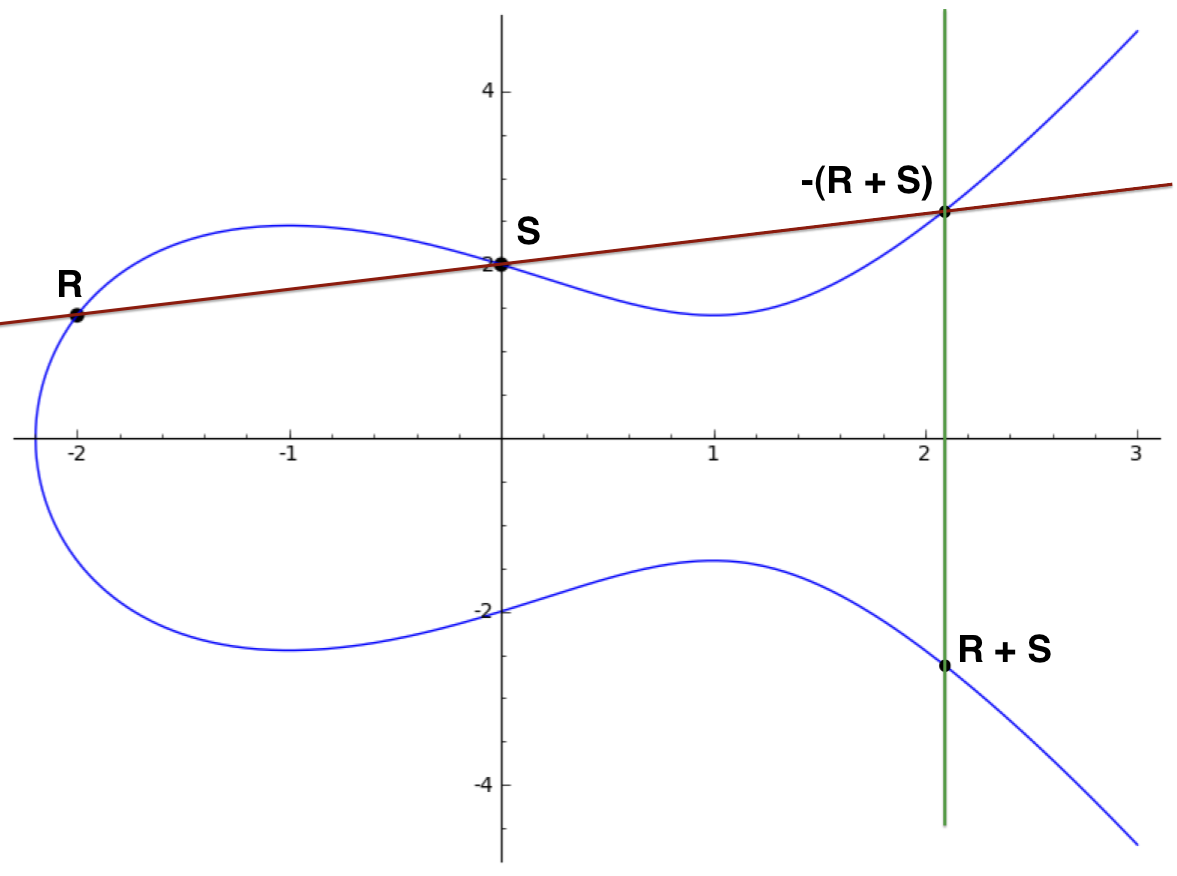
\includegraphics[scale=0.5]{figures/w_ells.png}
  \caption{$\ell_1$ and $\ell_2$ over a Weierstrass curve}
  \label{fig:w_ells}
\end{figure}

We can see the above claim that $g_{R, S} = \sfrac{\ell_1}{\ell_2}$ since
\[
div(\ell_1) = (R) + (S) + (-(R + S)) - 3(\mathcal{O})
\]
    because it has zeroes at $R$, $S$, and $-(R + S)$; since principal divisors
    have degree zero ($E$ is a smooth curve; see
    \cite{silverman2009arithmetic}, section II), we know that $\ell_1$ must
    have $\mathcal{O}$ as a pole of order three.
Similarly,
\[
div(\ell_2) = (-(R + S)) + (R + S) - 2(\mathcal{O})
\]
    since it intersects $E$ only at $R + S$, $-(R + S)$, and $\mathcal{O}$.
Finally,
\begin{align*}
div\left(\frac{\ell_1}{\ell_2}\right)
    &=  (R) + (S) + (-(R + S)) - 3(\mathcal{O}) -
            [(R + S) + (-(R + S)) - 2(\mathcal{O})]\\
    &=  (R) + (S) + (R + S) - (\mathcal{O})\\
    &=  div(g_{R, S})
\end{align*}
    as claimed.

This leads us to defining \textit{Miller functions} which arise in Miller's
    iterative algorithm for computing $\tau_n$.
We compute the needed $f$ with $div_P(f) = n(P) - n(\mathcal{O})$ with a take
    on the familiar ``double-and-and'' routine.
At each iteration we have some intermediate function $f_i$ with divisor $i(P) -
    (iP) - (i - 1)(\mathcal{O})$; after we complete our iterations, we have $f$
    since $nP = \mathcal{O}$.
This gives us Algorithm \ref{alg:miller}.

\begin{Algorithm}
\caption{Miller's Algorithm for computing $\tau_n$}
\label{alg:miller}
\begin{algorithmic}
    \Function{Miller}{$P, Q$}
        \State $f \gets 1$
        \State $R \gets P$
        \For{$i \gets k - 2 \texttt{ downto } 0$}
            \State $f \gets f^2 \cdot g_{R,R}(Q)$
            \State $R \gets 2R$ \Comment{Doubling Step}
            \If{$n_i = 1$}
                \State $f \gets f \cdot g_{R, P}(Q)$
                \State $R \gets R + P$ \Comment{Adding Step}
            \EndIf
        \EndFor
        \State $f \gets f^{\sfrac{(q^k - 1)}{n}}$
        \State \Return $f$
    \EndFunction
\end{algorithmic}
\end{Algorithm}

This algorithm is very efficient and the Weierstrass implementation has a nice
    geometric intuition behind it---the ``chord and tangent'' rule.
To compute pairings for a given normal form of an elliptic curve, it's enough
    to figure out what a Miller function looks like for that form, since this
    function ``forms the backbone for pairing computation.''
    \cite{das2008pairing}
Ergo in order to implement this for Edwards curves, we'll need a way to compute
    some Miller function $g_{R,S}$ with $div(g_{R,S}) = (R) + (S) - (R + S) -
    (\mathcal{O})$. 
So far pairing computations in the Edwards arena have been done for twisted
    Edwards curves, since they cover more cases of elliptic curves.
In trying to find Miller functions for binary Edwards curves, my research
    followed the same route that work has for twisted ones, beginning with the
    work of Das and Sarkar \cite{das2008pairing}.

\bodysection{Following Das \& Sarkar}

In \cite{das2008pairing}, the authors give a way of explicitly evaluating a
    pairing over twisted Edwards curves by using the birational map to and from
    a more familiar normal form.
We do the same here, but for binary Edwards curves.\footnote{In what follows,
    we shift our notation slightly to follow that of \cite{das2008pairing}
    instead of \cite{arene2011faster} since it makes our work slightly easier
    in the current setting.}

Let $\Phi$ be the birational map\footnote{It's really a group isomorphism when
    we extend it to the neutral elements, but nobody computes the pairing of a
    neutral element with another point in practice anyway.} from our binary
    Edwards curve $E$ to the corresponding Weierstrass curve
\[
W: v^2 + uv = u^3 + a_2u^2 + a_6
\]
Following the notation and work from \cite{moloneyefficient}, $\Phi$ is given
    by
\[
u = \sqrt{a_6}\left(\frac{(X + Y) Z}{d_1XY + d_1^2(X + Y)Z}\right)
\qquad
v = \sqrt{a_6}\left(\frac{(b + 1)XZ + bYZ}{d_1XY + d_1^2(X + Y)Z} + 1 +
    \frac{1}{d_1}\right)
\]
    where $b$ is chosen such that $b^2 + b = d_1^2 + d_2 + a_2$; i.e., $b$ is
    the half trace of $d_1^2 + d_2 + a_2$ (assuming that the degree $n$ of our
    binary field $\mathbb{F}_{2^n}$ is odd).
We also have $\Phi^{-1}: W \to E$ given by the projective coordinates
\begin{align*}
X   &=  d_1(bu + v + (d-1^2 + d_1)(d_1^2 + d_1 + d_2))\\
Y   &=  X + d_1u\\
z   &=  u^2 + d_1u + d_1^2(d_1^2 + d_1 + d_2)
\end{align*}

In order to calculate the pairing of $P_1$ and $P_2$ on $E$, we need to find a
    point $P_3$ and a rational function $h \in \mathbb{F}_{2^n}(E)$ such that
\[
\textrm{div}(h) = (P_1) + (P_2) - (P_3) - \mathcal{O}
\]
To do so, we'll map our points to $Q_1, Q_2, Q_3 \in W$ via $\Phi$, use the
    function
\[
g(u, v)
    =   \frac{\ell_1(u, v)}{\ell_2(u, v)}
    =   \frac{v + \lambda u + \theta}{u + u_3}
\]
    for lines $\ell_1$ through $Q_1$ and $Q_2$ and $\ell_2$ through $Q_3$ and
    $-Q_3$, then map back to $E$ via $\Phi^{-1}$.
The values $\lambda$ and $\theta$ are the slope and intercept of $\ell_1$,
    which is given via straight calculation.
Putting it all together, we have the following

\begin{thm}\label{thm:miller}
Let $E$ be a binary Edwards curve over $\mathbb{F}_{2^n}$ for $n$ odd, and $P_1
    = (X_1 : Y_1 : Z_1)$ and $P_2 = (X_2 : Y_2 : Z_2)$ be two points on $E$
    with sum $P_3 = (X_3 : Y_3 : Z_3)$.
Then the Miller function $h(x, y)$ such that
\[
\textrm{div}(h) = (P_1) + (P_2) - (P_3) - \mathcal{O}
\]
    is given by $\sfrac{N}{D}$, where
\[
D =
    (u1 + u2)
    (u_{3}  d_{1}  (d_{1} X Z + d_{1} Y Z + X Y) + \sqrt{a_6}  Z  (X + Y))
\]
    and the value of $N$ depends on whether $P_1$ and $P_2$ are equal:
\begin{enumerate}
\item   If $P_1 \ne P_2$, then 
\begin{align*}
N   &= Z  (X + Y)  d_{1}^{2}  (v_{1} u_{2} + u_{1} v_{2} + u_{1}
        \sqrt{a_6} + u_{2}\sqrt{a_6})\\
    &+ \sqrt{a_6}  (u_{1} + u_{2})  d_{1}  (X Y + X Z + Y Z)\\
    &+ Y  X  d_{1}  (v_{1} u_{2} + u_{1} v_{2})\\
    &+ \sqrt{a_6} (X Z u_{1} b + Y Z u_{1} b + X Z u_{2} b + Y Z u_{2} b\\
    &+ X Y u_{1} + X Z u_{1} + X Z v_{1} + Y Z v_{1} + X Y u_{2} + X Z u_{2} \\
    &+ X Z v_{2} + Y Z v_{2})\\
\end{align*}
\item If $P_1 = P_2$, then
\begin{align*}
N   &= u_{1}  Z  (X + Y)  d_{1}^{2}  (u_{1}^{2} + \sqrt{a_6})\\
    &+ u_{1}  d_{1}  (X Y u_{1}^{2} + X Y \sqrt{a_6} + X Z \sqrt{a_6} + Y Z
        \sqrt{a_6})\\
    &+  \sqrt{a_6}  (X Z u_{1}^{2} + Y Z u_{1}^{2} + X Z u_{1} b + Y Z u_{1} b
        + X Y u_{1} + X Z u_{1} + X Z v_{1} + Y Z v_{1})
\end{align*}
\end{enumerate}
\end{thm}

\begin{proof}
Given $\Phi(X, Y, Z) = (u, v)$ via the definition above, our function $h$ is
    $g\left(\Phi^{-1}(u, v)\right)$ per \cite{das2008pairing}.
That is, we have
\[
h
    =   g\left(
        \sqrt{a_6}\left(\frac{(X + Y) Z}{d_1XY + d_1^2(X + Y)Z}\right)
        ,
        \sqrt{a_6}\left(\frac{(b + 1)XZ + bYZ}{d_1XY + d_1^2(X + Y)Z} + 1 +
            \frac{1}{d_1}\right)
        \right)
\]
    which is equal to
\begin{equation}\label{eq:g_miller}
\frac{
    \sqrt{a_6}\left(
        \left[
            1 + \frac{1}{d_1} + \frac{(b + 1)XZ + bYZ}{d_1XY + d_1^2(X + Y)Z}
        \right]
        + \lambda\left[
            \frac{(X + Y)Z}{d_1XY + d_1^2(X + Y)Z}
        \right]
    \right) + \theta
}{
    \sqrt{a_6}\left[
        \frac{(X + Y)Z}{d_1XY + d_1^2(X + Y)Z} +
        \frac{(X_3 + Y_3)Z_3}{d_1X_3Y_3 + d_1^2(X_3 + Y_3)Z_3}
    \right]
}
\end{equation}
    where $\lambda$ and $\theta$ are determined by the line $\ell_1$.
Observe that if $P_1 \ne P_2$, then $\lambda$ is the slope of the line between
    them; if, on the other hand, $P_1 = P_2$, then it's the slope of the
    tangent line at $P_1$.
In either case, $\theta = v_1 + \lambda u_1$.

If $P_1 \ne P_2$, a straightforward calculation yields
\begin{equation}\label{eq:lam1}
\lambda = \frac{v_2 + v_1}{u_2 + u_1}
\end{equation}
    (since we're in characteristic two, addition and subtraction are the same).
If not, we use implicit differentiation on the equation for $W$ to find
    $\lambda = \frac{dv}{du}$:
\begin{align}\label{eq:lam2}
v^2 + uv = u^3 + a_6u^2 + a_2
    &\implies   2v\lambda + u\lambda + v = 3u^2 + 2a_6u\notag\\
    &\implies   \lambda\big\vert_{(u_1, v_1)} = \frac{u_1^2 + v_1}{u_1}
\end{align}
    remembering again that we're in characteristic two.

Replacing $\lambda$ with (\ref{eq:lam1}) and (\ref{eq:lam2}), in turn, and
    taking $\theta = v_1 + \lambda u_1$ yields the desired result after some
    tedious calculation.
Rather than show all the work, we include the following Sage script that
    will do the heavy lifting for us:
\lstinputlisting[caption={Calculations for binary Edwards Pairings},language=Python]{listings/calc.sage}
\end{proof}


\bodysection{Directions for Future Work}

Clearly the preceding theorem, though perfectly adequate, leaves something to
    be desired; a more elegant, cleaner solution for the Miller function would
    be nice.
The most clear way to such a solution, as evidenced by \cite{arene2011faster}
    and \cite{lipairing}, is to get a better understanding of the geometry of
    binary Edwards curves.
To that end, we show how to extend one of the theorems of
    \cite{arene2011faster} from twisted Edwards curves to binary Edwards
    curves.
We intend this theorem to be a stepping stone towards a full result similar to
    the main idea of \cite{arene2011faster}, wherein they give a new geometric
    formulation of the twisted Edwards curve group law (among many other
    interesting results).

In \cite{arene2011faster}, the authors give a new interpretation of the group
    law similar in its geometric flavor to the familiar ``chord-and-tangent''
    law of Weierstrass curves.
They show that the sum of two points on a twisted Edwards curve $E_{T, a, d}$
    can be given by a special conic: quoting their \textit{Remark 3}, ``we see
    that $P_1 + P_2$ is obtained as the mirror image with respect to the
    $y$-axis of the eighth intersection point of $E_{T, a,d}$ and the conic
    passing through $\Omega_1, \Omega_2, \mathcal{O}^\prime, P_1$, and $P_2$,''
    where $\Omega_1$ and $\Omega_2$ are the two points at infinity $(1 : 0 :
    0)$ and $(0 : 1 : 0)$, respectively, and $\mathcal{O}^\prime$ is the point
    $(0, -1)$ of order 2.
We offer an analogous result to their main theorem (1) that paves the way for
    their geometric interpretation in the hopes that it will inspire similar
    results for binary Edwards curves.

Let $\mathcal{O}^\prime = (1, 1) = (1 : 1 : 1)$; recall that this point has
    order 2.
Furthermore, let $\varphi(X, Y, Z) = c_{X^2}X^2 + c_{Y^2}Y^2 + c_{Z^2}Z^2 +
    c_{XY}XY + c_{XZ}XZ + c_{YZ}YZ \in K[X, Y, Z]$ be a homogeneous polynomial
    of degree 2 and $C: \varphi(X, Y, Z) = 0$ be the associated plane (possibly
    degenerate) conic.
Like in \cite{arene2011faster}, since the points $\Omega_1, \Omega_2,$ and
    $\mathcal{O}^\prime$ do not lie on a line, a conic $C$ passing through
    these points cannot be a double line and $\varphi$ represents $C$ uniquely
    up to multiplication by a scalar.
By evaluating $\varphi$ at $\Omega_1, \Omega_2,$ and $\mathcal{O}^\prime$, we
    get the following:
\begin{align*}
\Omega_1:\qquad &\varphi(1 : 0 : 0) = c_{X^2}\\
\Omega_2:\qquad &\varphi(0 : 1 : 0) = c_{Y^2}\\
\mathcal{O}^\prime:\qquad&\varphi(1, 0, 0) = c_{X^2} + c_{Y^2} + c_{Z^2} +
                                             c_{XY} + c_{XZ} + c_{YZ}
\end{align*}
Hence $c_{X^2} = c_{Y^2} = 0$ and $c_{Z^2} = c_{XY} + c_{XZ} + c_{YZ}$.
Therefore $C$ must have the form:
\begin{equation}\label{eq_C}
c_{XY}(XY + Z^2) + c_{XZ}(XZ + Z^2) + c_{YZ}(YZ + Z^2)
\end{equation}
Next we have the following analogous result to Theorem 1 of
    \cite{arene2011faster}:

\begin{thm}\label{thm:arene}
Let $E_{B, d_1, d_2}$ be a binary Edwards curve over $K$ and let $P_1 = (X_1 :
    Y_1 : Z_1)$ and $P_2 = (X_2 : Y_2 : Z_2)$ be two affine, not necessarily
    distinct, points on $E_{B, d_1, d_2}(K)$.
Let $C$ be the conic passing through $\Omega_1, \Omega_2, \mathcal{O}^\prime,
    P_1,$ and $P_2$ which must have the form (\ref{eq_C}).
If some of the above points are equal, we consider $C$ and $E_{B, d_1, d_2}$
    to intersect with at least that multiplicity at the corresponding point.
Then the coefficients in (\ref{eq_C}) of the equation $\varphi$ of the conic
    $C$ are uniquely determined (up to scalars) as follows:
\begin{enumerate}
\item
If $P_1 \ne P_2, P_1 \ne \mathcal{O}^\prime,$ and $P_2 \ne \mathcal{O}^\prime$,
    then
\begin{align*}
c_{XY}  &=Z_1Z_2\left[X_1(Y_2 + Z_2) + Y_1(X_2 +Z_2) + Z_1(X_2 + Y_2)\right]\\
c_{XZ}  &=Y_1Z_2(X_1Y_2 + X_1Z_2 + Z_1Z_2) + Y_2Z_1(Y_1X_1 + Z_1X_1 + Z_1Z_2)\\
c_{YZ}  &=X_1Z_2(Y_1X_2 + Y_1Z_2 + Z_1Z_1) + X_2Z_1(X_1Y_2 + Z_1Y_2 + Z_1Z_2)
\end{align*}
\item
If $P_1 \ne P_2 = \mathcal{O}^\prime$, then $c_{XY} = Z_1, c_{XZ} = Z_1,$ and
    $c_{YZ} = X_1 $
\item
If $P_1 = P_2$, then
\begin{align*}
c_{XY}  &=  X_1^2Y_1 + X_1Y_1^2 + d_1X_1Z_1^2 + X_1^2Z_1 + d_1Y_1Z_1^2 +
            Y_1^2Z_1 + X_1Z_1^2 + Y_1Z_1^2\\
c_{XZ}  &=  X_1^2Y_1 + d_1Y_1^2Z_1 + X_1Y_1^2 + d_1X_1Z_1^2 + X_1^2Z_1\\
        &+ d_1Y_1Z_1^2 + X_1Y_1Z_1 + d_1Z_1^3 + Y_1Z_1^2\\
c_{YZ}  &=  d_1X_1^2Z_1 +d_2X_1^2Z_1 + d_2Y_1^2Z_1 + X_1^2Z_1 + d_1Z_1^3 +
            X_1Z_1^2
\end{align*}
\end{enumerate}
\end{thm}

\begin{proof}
We tackle each case separately.
\begin{enumerate}
\item
If the points $P_1$ and $P_2$ are distinct, evaluating equation \ref{eq_C} at
    the two points yields two linear equations in the coefficients:
\begin{align*}
c_{XY}(X_1Y_1 + Z_1^2) + c_{XZ}(X_1Z_1 + Z_1^2) + c_{YZ}(Y_1Z_1 + Z_1^2) &= 0\\
c_{XY}(X_2Y_2 + Z_2^2) + c_{XZ}(X_2Z_2 + Z_2^2) + c_{YZ}(Y_2Z_2 + Z_2^2) &= 0
\end{align*}
Since we're working in projective coordinates, two equations is enough to
    uniquely determine the three unknowns, and we get the following solutions:
\begin{align*}
c_{XY}
    &=  \begin{vmatrix}
        X_1Z_1 + Z_1^2  &   Y_1Z_1 + Z_1^2\\
        X_2Z_2 + Z_2^2  &   Y_2Z_2 + Z_2^2
        \end{vmatrix}\\
    &=  (X_1Z_1 + Z_1^2)(Y_2Z_2 + Z_2^2) + (X_2Z_2 + Z_2^2)(Y_1Z_1 + Z_1^2)\\
    &=  Z_1Z_2\left[X_1(Y_2 + Z_2) + Y_1(X_2 +Z_2) + Z_1(X_2 + Y_2)\right]\\
c_{XZ}
    &=  \begin{vmatrix}
        X_1Y_1 + Z_1^2  &   Y_1Z_1 + Z_1^2\\
        X_2Y_2 + Z_2^2  &   Y_2Z_2 + Z_2^2
        \end{vmatrix}\\
    &=  (X_1Y_1 + Z_1^2)(Y_2Z_2 + Z_2^2) + (X_2Y_2 + Z_2^2)(Y_1Z_1 + Z_1^2)\\
    &=  X_1^2Y_1 + d_1Y_1^2Z_1 + X_1Y_1^2 + d_1X_1Z_1^2 + X_1^2Z_1\\
    &+ d_1Y_1Z_1^2 + X_1Y_1Z_1 + d_1Z_1^3 + Y_1Z_1^2\\
c_{YZ}
    &=  \begin{vmatrix}
        X_1Y_1 + Z_1^2  &    X_1Z_1 + Z_1^2\\
        X_2Y_2 + Z_2^2  &    X_2Z_2 + Z_2^2
        \end{vmatrix}\\
    &=  (X_1Y_1 + Z_1^2)(X_2Z_2 + Z_2^2) + (X_2Y_2 + Z_2^2)(X_1Z_1 + Z_1^2)\\
    &=  d_1X_1^2Z_1 +d_2X_1^2Z_1 + d_2Y_1^2Z_1 + X_1^2Z_1 + d_1Z_1^3 + X_1Z_1^2
\end{align*}
    as claimed.

\item
Note that $C$ is tangent to the curve $E_{B, d_1, d_2}$ at the point
    $\mathcal{O}^\prime$ if and only if $0 = \left(\sfrac{\partial\varphi}
    {\partial x}\right)(1 : 1 : 1) = c_{XY} + c_{XZ}$, i.e. iff $c_{XY} =
    c_{XZ}$.
Then
\[
\varphi
    =   c_{XY}(XY + Z^2 + XZ + Z^2) + c_{YZ}(YZ + Z^2)
    =   (Y + Z)(c_{XY}X + c_{YZ}Z)
\]
Since $P_1 \ne \mathcal{O}^\prime$, it doesn't lie on the line $Y + Z = 0$, so
    $c_{XY}X_1 + c_{YZ}Z_1 = 0$.
Then together $c_{XY} = c_{XZ}$ and $c_{XY}X_1 = c_{YZ}Z_1$ imply the result.

\item
In the final case, let $Z = Z_1 = 1$ in our equations.
The tangent vectors at $P_1 = (X_1 : Y_1 : 1) = (X_1, Y_1)$ of
    $E_{B, d_1, d_2}$ and $C$ are
\[
\begin{pmatrix}
    \sfrac{\partial E}{\partial Y} \\ \sfrac{\partial E}{\partial X}
\end{pmatrix}
=   
\begin{pmatrix}
d_1 + X_1 + X_1^2 \\ d_1 + Y_1 + Y_1^2
\end{pmatrix}
\qquad
\begin{pmatrix}
    \sfrac{\partial C}{\partial Y} \\ \sfrac{\partial C}{\partial X}
\end{pmatrix}
\begin{pmatrix}
c_{XY}X_1 + c_{YZ} \\ c_{XY}Y_1 + c_{XZ}
\end{pmatrix}
\]
    (note that we can drop the usual negative signs because $\textrm{char}(K) =
    2$).
These vectors are collinear if and only if
\begin{align*}
0
    &=  \begin{vmatrix}
        d_1 + X_1 + X_1^2   &   c_{XY}X + c_{YZ}\\
        d_1 + Y_1 + Y_1^2   &   c_{XY}Y + c_{XZ}
        \end{vmatrix}\\
    &=  c_{XY}(d_1Y_1 + X_1Y_1 + X_1^2Y_1 + d1X_1 + X_1Y_1 + X_1Y_1^2)\\
    &+c_{XZ}(d_1 + X_1 + X_1^2) + c_{YZ}(d_1 + Y_1 + Y_1^2)\\
    &=  c_{XY}(d_2(X_1^2 + Y_1^2) + X_1^2Y_1^2) +
        c_{XZ}(d_1 + X_1 + X_1^2) +
        c_{YZ}(d_1 + Y_1 + Y_1^2)
\end{align*}
    using the curve equation to simplify.
We also know that
\[
0   =   \varphi(X_1, Y_1, 1)
    =   c_{XY}(X_1Y_1 + 1) + c_{XZ}(X_1 + 1) + c_{YZ}(Y_1 + 1)
\]
These two equations can be solved in the same manner as our work in the first
    case, yielding
\begin{align*}
c_{XY}
    &=  \begin{vmatrix}
        d_1 + X_1 + X_1^2   &   d_1 + Y_1 + Y_1^2\\
        X_1 + 1   &   Y_1 + 1
        \end{vmatrix}\\
    &=  d_1(X_1 + Y_1) + X_1 + Y_1 + X_1^2 + Y_1^2 + X_1^2Y_1 + X_1Y_1^2\\
    &=  (X_1 + Y_1)(X_1Y_1 + X_1 + Y_1 + d_1 + 1)
\end{align*}
    for the first coefficient,
\begin{align*}
c_{XZ}
    &=  \begin{vmatrix}
        d_2(X_1^2 + Y_1^2) + X_1^2Y_1^2 &   d_1 + Y_1 + Y_1^2\\
        X_1Y_1 + 1  &   Y_1 + 1
        \end{vmatrix}\\
    &=  d_1(X_1Y_1 + 1) + d_2(X_1^2Y_1 + Y_1^3 + X_1^2 + Y_1^2) + X_1^2\\
    &+ Y_1^2 + X_1Y_1^2 + X_1Y_1^3 + Y_1 + Y_1^2 + X_1^2Y_1^3\\
    &=  X_1^2Y_1 + d_1Y_1^2 + X_1Y_1^2 + d_1X_1 + X_1^2 + d_1Y_1 + X_1Y_1 + d_1
        + Y
\end{align*}
    for the second, and
\begin{align*}
c_{YZ}
    &=  \begin{vmatrix}
        d_2(X_1^2 + Y_1^2) + X_1^2Y_1^2 &   d_1 + X_1 + X_1^2\\
        X_1Y_1 + 1  &   X_1 + 1
        \end{vmatrix}\\
    &=  d_1(X_1Y_1 + 1) + d_2(X_1^3 + X_1^2 + X_1Y_1^2 + Y_1^2) + X_1^34Y_1^2\\
    &+ X_1^2Y_1^2 + X_1^2Y_1 + X_1^3Y_1 + X_1 + X_1^2\\
    &=  d_1X_1^2 + d_2X_1^2 + d_2Y_1^2 + X_1^2 + X_1 + d_1
\end{align*}
    for the third, using the curve equation to simplify.
Homogenizing yields the stated result.
Note that the same formulas work if $P_1 = \mathcal{O}^\prime$, since then we
    still have $\varphi = 0$.\qedhere
\end{enumerate}
\end{proof}

Unfortunately, it's not entirely clear where to go from here; the geometry of
    twisted Edwards curves is different from the geometry of binary Edwards
    curves.
Moreover, though working in characteristic two has some benefits to arithmetic,
    more often than not it seems to complicate calculations.
Therefore, theorem \ref{thm:arene} is offered as a possible starting point for
    future research instead of an end in and of itself.
If we were to continue to mirror the progression of results for pairings on
    twisted Edwards curves, the next step would be to expand on a result
    similar to \cite{arene2011faster}'s to get one similar to
    \cite{lipairing}'s.
Again, because the geometry of binary Edwards curves differs so much from that
    of twisted means the results of this paper don't directly apply, but they
    do offer an intriguing possibility for another direction.
Such a result would involve not only reinterpreting the geometry of binary
    Edwards curves, but would also involve working in extended coordinates
    (four instead of the usual three for projective space).
